
% Auriga theme
% https://github.com/anishathalye/auriga

\documentclass[14pt,aspectratio=169]{beamer}
\usepackage{pgfpages}
\usepackage{amsmath}
\usepackage{fancyvrb}
\usepackage{tikz}
\usetikzlibrary{arrows.meta, positioning, quotes}
\usepackage{pgfplots}

% \ifnotes
% \setbeamertemplate{note page}[plain]
% \setbeameroption{show notes on second screen=right}
% \fi

\usetheme{auriga}
\usecolortheme{auriga}

% define some colors for a consistent theme across slides
\definecolor{red}{RGB}{181, 23, 0}
\definecolor{blue}{RGB}{0, 118, 186}
\definecolor{gray}{RGB}{146, 146, 146}

\title{Universidad Nacional de Córdoba (UNC) \\ Maestría en Economía
  Pública y Políticas Económicas, Sociales y Regionales (MEPPESR) \\
  La Economía Politica de las Políticas
  Públicas}
\subtitle{Clase 4}
\author{\underline{Sebastian Freille} \inst{1}}
\institute[IEF (FCE-UNC)]{\inst{1} Instituto de Economía y Finanzas (FCE-UNC)}
\date{}



\AtBeginSection[]{
    \begin{frame}
    \vfill
    \centering
    \begin{beamercolorbox}[sep=8pt,center,shadow=true,rounded=true]{title}
        \usebeamerfont{title}\insertsectionhead\par%
    \end{beamercolorbox}
    \vfill
    \end{frame}
}


\begin{document}
\maketitle


\section{Actores en el proceso de la política pública}


% \begin{frame}\frametitle{Preguntas}
%     \begin{itemize}\itemsep 10pt
%       \item ¿Quíenes son los diferentes actores involucrados en el
%         diseño de la política pública?
%         \item ¿Qué tipologías de actores existen y cuáles son las
%           características?
%           \item ¿Qué grado de homogeneidad en los
%             intereses/preferencias existen entre los diferentes tipos
%             de actores?
%            \item ¿Qué margen existe para la aparición de políticas de
%              consenso que contribuyan a la estabilidad de las políticas?
%     \end{itemize}
%   \end{frame}


  \begin{frame}\frametitle{Proceso de Formulación de Políticas (PFP)}
    \begin{itemize}
    \item El proceso de formulación de políticas (PFP)
      $\longrightarrow$ juego dinámico entre actores que interactúan
      en escenarios
      \item Constituciones asignan el rol de la
        formulación de políticas a tres ramas separadas: ejecutiva,
        legislativa y judicial (dimensión horizontal).
        \item En algunos casos particulares, también existe una
          dimensión vertical (federalismo) de las instituciones
          $\longrightarrow$ división de roles entre niveles de gobierno
          \item Muchos actores no oficiales
            participan del diseño, implementación y
            evaluación de las políticas públicas. 
        \end{itemize}
        \end{frame}


        \begin{frame}\frametitle{Tipificación de actores en el PFP}
          \begin{itemize}
      \item Estos actores pueden ser tipificados y categorizados de
        diferentes formas:
        \begin{itemize}
          \item Actores \textbf{formales} e
        \textbf{informales}. Entre los primeros están los partidos
        políticos, los presidenes, el gabinete, la Legislatura y la
        burocracia. Entre los segundos, se encuentran las empresas,
        los movimientos sociales, y los medios de comunicación. En el primer caso, sus roles y funciones en el PFP están
          contemplados en la Constitución y otras leyes. En el segundo
          caso, no tienen un rol formal pero pueden ejercer gran
          influencia.
          \item Actores \textbf{institucionales} y \textbf{no
              institucionales}
            \item Actores según rama: \textbf{ejecutivo},
              \textbf{legislativo}, y \textbf{judicial}.
              \end{itemize}
            \end{itemize}
    \end{frame}


    \begin{frame}\frametitle{Clasificación de actores}
      \begin{itemize}
      \item Gobierno
        \begin{itemize}
        \item Poder ejecutivo
        \item Poder legislativo
        \item Poder judicial
          \end{itemize}
        \item Burocracia
        \item Grupos de interés
          \begin{itemize}
          \item Empresas
          \item Asociaciones y organizaciones del tercer sector
          \item Medios de comunicación
          \end{itemize}
        \item Partidos políticos y votantes
        \end{itemize}
          \end{frame}

    
    \begin{frame}\frametitle{Proceso de Formulación de Políticas (PFP) (cont.)}
      \begin{block}{Políticas y proceso de formulación de políticas}
La política es lo que el Gobierno dice y hace sobre los problemas
percibidos. La formulación de políticas es cómo el Gobierno decide qué
se hará sobre los problemas percibidos. El proceso de formulación de
políticas es un proceso de interacción entre actores gubernamentales y
no gubernamentales; la política es el resultado de esa interacción
[Ripley and Franklin]
        \end{block}
      \end{frame}
    
    
% \begin{frame}\frametitle{Actores formales I}
%   \begin{block}{Partidos políticos}
% Los partidos políticos son la peor forma de participación política
% organizada, excepto por todas las demás [Osvaldo Hurtado, presidente
% de Ecuador]
%     \end{block}
%   \end{frame}


% \begin{frame}\frametitle{Actores formales I: Partidos políticos,
%     Legislaturas y Presidente}
%   \begin{itemize}\itemsep 10pt
%   \item Son tres actores protagónicos y esenciales del PFP. Su
%     importancia radica en que la naturaleza del sistema de partidos,
%     la estructura y funcionamiento de la Legislatura y los incentivos
%     y limitaciones del Presidente impactan en las características y
%     resultados de las políticas públicas.
%     \item Es importante estudiar la interacción entre estos actores
%       --en particular, interesa estudiar la interrelación entre el
%       Presidente y la Legislatura.
%       \item Capacidad de los Presidentes de llevar a cabo sus
%         programas de gobierno
%         \item En América Latina se ha cuestionado el presidencialismo
%           $\longrightarrow$ especialemnte cuando hay gobierno
%           dividido. 
%   \end{itemize}
%   \end{frame}

  \section{Gobierno}

  \subsection{Gobierno: Poder ejecutivo}
  
  \begin{frame}\frametitle{Poder ejecutivo}
    \begin{itemize}
\item En democracias modernas, se observa un amplio rango de
  sistemas entre dos esquemas opuestos: \textbf{presidencialismo} y
  \textbf{parlamentarismo}.
  \item Países latinoamericanos en general  regímenes
    presidencialistas; países europeos en su
    mayoría tienen sistema parlamentario
    \item Sistemas parlamentarios suelen asociarse a menor estabilidad
      que sistemas presidencialistas ya que los líderes suelen cambiar
      con mayor frecuencia --en República Checa, 4 líderes en 12 años;
      en Ucrania, 5 líderes en 15 años; Rajoy en España.  
% \item Pero estos cambios no suelen ser bruscos o traumáticos y no
%   implican una reorganización total del Gobierno. Esto lleva a que los
%   sistemas parlamentarios se consideran \textbf{flexibles} y los
%   presidencialistas \textbf{rígidos}. 
    \end{itemize}
    \end{frame}



    

 \begin{frame}\frametitle{Poder ejecutivo (cont.)}
   \begin{block}{Mirando la evidencia I}
Tomando datos de todas las democracias presidencialistas entre 1946 y
1996, varios autores muestran que los presidentes y los gobiernos
minoritarios no afectan la supervivencia de la democracia
     \end{block}
     \begin{block}{Mirando la evidencia II}
Tomando datos de gobiernos latinoamericanos entre 1978 y
2005, otros autores muestran que varios gobiernos minoritarios
--aquellos que controlan menos del 45\% del Congreso-
sufrieron interrupciones. Los gobiernos
minoritarios son hasta cinco veces más propensos a sufrir
interrupciones.
       \end{block}
      %  \begin{block}{El caso de Ecuador}
% Ningún presidente terminó su mandato desde el año 1996 hasta el año
% 2006 (año en que gana Correa). En ese período, hubo tres presidentes
% derrocados. En el 2008 se cambió la Constitución. 
%          \end{block}
     \end{frame}
    

 \begin{frame}\frametitle{Poder ejecutivo: Presidente}
\begin{itemize}
 \item ¿Qué determina la capacidad del Presidente de llevar a cabo
      su programa de gobierno? $\longrightarrow$ proporción de escaños
      controlados en la Legislatura. Dos situaciones.
      \item Si Presidente controla mayoría $\longrightarrow$ mayor
        facilidad para lograr programa de gobierno y mayor
        adaptabilidad de política públicas
        \item Si Presidente no controla mayoría $\longrightarrow$
          deben estructurar coaliciones que pueden ser de dos tipos:
          \begin{itemize}
          \item Coaliciones estables $\longrightarrow$ basadas en
            apoyo general y estable de minorías
            \item Coaliciones puntuales $\longrightarrow$ coaliciones
              diferentes para diferentes medidas y/o políticas
              públicas. 
            \end{itemize}          
      \end{itemize}
  \end{frame}
     
\begin{frame}\frametitle{Poder ejecutivo: Presidente (cont.)}
\begin{itemize}
\item ¿Qué incentivos afectan el comportamiento del Presidente?
\item Contexto institucional $\longrightarrow$ Presidente se
  interese por el bien público y políticas para mayorías; o por
  intereses particulares que benrfician a
  minorías poderosas
  \item Diferencias en incentivos explicadas por reglas
    electorales mientras que capacidad para transformar políticas
    depende de poderes otorgados institucionalmente
    \item Los poderes otorgados a los presidentes se clasifican en
      \textit{poderes constitucionales} y \textit{poderes
        partidistas}.  
\end{itemize}
\end{frame}


 

\begin{frame}\frametitle{Poder ejecutivo: Presidente (cont.)}
  \begin{itemize}
  \item Poderes constitucionales $\longrightarrow$ enmarcan las
    relaciones entre ejecutivo y legislativo. Pueden dividirse en:
    \begin{itemize}
    \item Poderes legislativos $\longrightarrow$ incluyen poder de
      veto total, veto parcial, el poder de aprobar decretos, el poder
      para convocar a un plebiscito. Si tiene poderes amplios, las
      políticas públicas reflejarán sus preferencias/intereses.
      \item Poderes no legislativos $\longrightarrow$ poder de
       nominar, nombrar y despedir funcionarios, ministros y
       jueces. Esto le permite cierto grado de influencia sobre los
       otros poderes
      \end{itemize}
   \item Poderes partidistas $\longrightarrow$ se relaciona con el
     grado de apoyo en el Congreso del Presidente --i.e. tamaño de su
     bloque y grado de disciplina partidaria
    \end{itemize}
  \end{frame}



\begin{frame}\frametitle{Poder ejecutivo: Presidente (cont.)}
 \begin{figure}[htbp]\vspace{0cm}
    \centering
    \includegraphics[scale=0.25]{presidentes1}
    \caption{Tasa de aprobación legislativa}
    \label{fig:1}
  \end{figure}
        \end{frame}

  
  
\begin{frame}\frametitle{Poder ejecutivo: Presidente (cont.)}
 \begin{figure}[htbp]\vspace{0cm}
    \centering
    \includegraphics[scale=0.25]{legislativo1}
    \caption{Tasa de aprobación legislativa}
    \label{fig:1}
  \end{figure}
        \end{frame}


  
  \begin{frame}\frametitle{Poder ejecutivo: Reglas electorales}
  \begin{itemize}
  \item Los Presidentes pueden ser elegidos de varias formas. Algunos
    de los sistemas más comunes son:
    \begin{itemize}
      \item Escrutinio mayoritario uninominal (``first past the
        post'') $\longrightarrow$ sistema más simple de
        mayoría/pluralidad. Cada persona vota por un sólo candidato y
        gana el que más votos recibe
    \item Sistema de dos vueltas (``two-round system'')
      $\longrightarrow$ se trata de un sistema con dos elecciones. La
      primera vuelta se suele definir por FPTP y la segunda por
      mayoría absoluta
      \item Voto único transferible (``single transferable vote'')
        $\longrightarrow$ se basa en la representación proporcional y
        voto de preferencia --el voto de un elector se asigna
        inicialmente a su candidato más preferido; pero si ese
        candidato hubiera sido elegido/eliminado esos votos se
        transfieren al candidato que sigue despues en la preferencia.
      \end{itemize}
    \end{itemize}
  \end{frame}


  \begin{frame}\frametitle{Poder ejecutivo: Reglas electorales (cont.)}
  \begin{itemize}\itemsep 15pt
  \item Por primera vez en la historia se usará este sistema en las
    primarias para elegir intendente (``mayor'') en la ciudad de Nueva
    York
    \item Una de las principales desventajas es la aparente dificultad
      para utilizar la boleta y el sistema de votación para evitar que
      el voto sea considerado inválido
      \item Varios países y gobiernos subnacionales han coqueteado con
        este sistema por cuanto permite, a priori, considerar toda la
        información de las preferencias de los votantes
    \end{itemize}
  \end{frame}


 \begin{frame}\frametitle{Poder ejecutivo: Reglas electorales (cont.)}
  \begin{figure}[htbp]\vspace{0cm}
    \centering
    \includegraphics[scale=0.5]{rank01}
    \caption{Ejemplo de boletas}
    \label{fig:1}
  \end{figure}
  \end{frame}


  \begin{frame}\frametitle{Poder ejecutivo: Reglas electorales (cont.)}
  \begin{figure}[htbp]\vspace{0cm}
    \centering
    \includegraphics[scale=0.5]{rank02}
    \caption{Ejemplo de boletas - Válidas}
    \label{fig:1}
  \end{figure}
  \end{frame}


  
  \begin{frame}\frametitle{Poder ejecutivo: Reglas electorales (cont.)}
  \begin{figure}[htbp]\vspace{0cm}
    \centering
    \includegraphics[scale=0.5]{rank03}
    \caption{Ejemplo de boletas - No válidas}
    \label{fig:1}
  \end{figure}
  \end{frame}

  

  \begin{frame}\frametitle{Poder ejecutivo: Reglas electorales (cont.)}
 \begin{figure}[htbp]\vspace{0cm}
    \centering
    \includegraphics[scale=0.5]{rank04}
    \caption{Ejemplo de boletas - No válidas}
    \label{fig:1}
  \end{figure}
        \end{frame}



  \begin{frame}\frametitle{Poder ejecutivo: Reglas electorales (cont.)}
 \begin{figure}[htbp]\vspace{0cm}
    \centering
    \includegraphics[scale=0.55]{electoralrules2}
    \caption{Voto único transferible}
    \label{fig:1}
  \end{figure}
        \end{frame}
        

 \begin{frame}\frametitle{Poder ejecutivo: Reglas electorales (cont.)}
  \begin{itemize}
  \item El método de elección del Presidente incide en el apoyo
    electoral del mismo y sobre la necesidad de formar o no
    coaliciones para gobernar $\longrightarrow$ la necesidad de armar
    coaliciones para gobernar crea restricciones 
    \item Otro aspecto relevante es si las elecciones
      ejecutivas/legislativas son \textbf{concurrentes} y si existen
      elecciones legislativas de medio término.
      \item Cuando hay elecciones concurrenes para ejecutivo y
        legislativo, el partido del presidente tiene posibilidad de
        recibir mas votos --efecto ``coattail''.
      \end{itemize}
      \end{frame}

      
      \begin{frame}\frametitle{Poder ejecutivo: Reglas electorales (cont.)}
        \begin{itemize}
      \item \textbf{nominación de
            candidatos presidenciales}. La selección puede ser
          \textit{centralizada} --elites partidarias- o
          \textit{descentralizada}
          \item Otro tema central para los
            incentivos del presidente es la \textbf{longitud del
              mandato}. Condicionado por
            las disposiciones en relación a la \textit{longitud del
              período} y las \textit{disposiciones sobre
              reelección}. Políticas estarán condicionadas
            a las propuestas en la campaña de reelección.
            \item Si no puede reelegirse, tiene menor incentivo a ser
              fiscalmente responsable $\longrightarrow $ ``teoría del
              pato rengo''. 
                \end{itemize}
  \end{frame}
        
  
    \begin{frame}\frametitle{Poder ejecutivo: Reglas electorales (cont.)}
 \begin{figure}[htbp]\vspace{0cm}
    \centering
    \includegraphics[scale=0.25]{electoralrules1}
    \caption{¿Qué sistema se usa para elegir al Presidente?}
    \label{fig:1}
  \end{figure}
        \end{frame}


 \begin{frame}\frametitle{Poder ejecutivo: El Gabinete}
  \begin{itemize}
  \item Aunque no está tan directamente involucrado con el \textit{diseño} de
    la política pública, si juega de lleno cuando se trata de la
    \textit{implementación}.
  \item Dos aspectos sobresalen aquí:
    \begin{itemize}
    \item Proceso de formación del gabinete $\longrightarrow$ sisemas
      mayoritarios tienden a tener gabinetes compactos; sistemas de
      coalición tienen a tener gabinetes mixtos --i.e funcioarios
      radicales y de CC en gabinete de Cambiemos. Evidencia: a
      menor número de partidos en gabinete menor el
      nivel de gasto público. 
      \item Estabilidad del gabinete $\longrightarrow$ no sólo tiene
        que ver con la estabilidad de nombres sino también con la
        estructura de gobierno (Ley Orgánica) --i.e alta inestabilidad
        de gabinete asociada con alta inestabilidad de políticas. 
      \end{itemize}
            \end{itemize}
      \end{frame}



      
\begin{frame}\frametitle{Poder ejecutivo: El gabinete}
 \begin{figure}[htbp]\vspace{0cm}
    \centering
    \includegraphics[scale=0.3]{gabinete1}
    % \caption{Inestabilidad del gabinete}
    \label{fig:1}
  \end{figure}
        \end{frame}


        
 \subsection{Gobierno:  Poder legislativo}

 
  \begin{frame}\frametitle{Poder legislativo}
    \begin{itemize}
    \item En términos generales, la legislatura ayuda a reducir la
      volatilidad de las políticas y a representar mejor las
      preferencias ciudadanas.
      \item Es importante caracterizar las \textbf{reglas
          electorales} --reglas de acceso a la legislatura y de
        nominación-- y las \textbf{reglas de la estructura
          legislativa} --hacen al funcionamiento de la legislatura y
        roles de los comités.
        \item Legislatura está condicionada por los
          poderes otorgados al presidente pero dependiendo de su
          diseño institucional podrá exacerbar o compensar ciertas características
    \end{itemize}
    \end{frame}


    \begin{frame}\frametitle{Poder legislativo: Reglas electorales}
    \begin{itemize}
    \item El \textbf{método de elección} de los representantes es uno
      de los principales determinantes del número de actores y de sus
      incentivos.
      \item El método de elección puede ser \textit{directo} o
        \textit{indirecto}. El método directo tiende a alinear los
        intereses ciudadanos con los de los legisladores; el método
        indirecto tiende a alinear a ejecutivo con legislativo
        \item Pero aún cuando se elijan de manera directa, existen
          muchas variantes aqúi que conviene resaltar. 
    \end{itemize}
    \end{frame}


\begin{frame}\frametitle{Poder legislativo: Reglas electorales (cont.)}
 \begin{figure}[htbp]\vspace{0cm}
    \centering
    \includegraphics[scale=0.25]{electoralrules3}
    \caption{¿Qué sistema se usa para elegir al Congreso?}
    \label{fig:1}
  \end{figure}
        \end{frame}


    
    \begin{frame}\frametitle{Poder legislativo: Reglas electorales (cont.)}
    \begin{itemize}
    \item En primer lugar, importa el \textbf{tamaño (magnitud) del
        distrito}. Existen básicamente dos sistemas aquí:
      \begin{itemize}\itemsep 5pt
      \item Sistemas de distritos uninominales $\longrightarrow$ cada
        distrito es representado por \textbf{un} solo legislador
        \item Sistemas de distritos plurinominales $\longrightarrow$
          cada distrito es representado por \textbf{varios} legisladores
        \end{itemize}
        \item Dependiendo del tipo de sistema, los países tendrán
          diferentes estructuras partidarias representadas en la
          legislatura --i.e. número efectivo de partidos 
    \end{itemize}
    \end{frame}
        

% \begin{frame}\frametitle{Las ``leyes'' de Duverger}
%  \begin{block}{Ley 1}
% Los sistemas de votación por mayoría en una elección conducen a un sistema bipartidista
% \end{block}
% \begin{block}{Ley 2}
% Los sistemas de votación por representación proporcional conducen a un
% sistema multipartidista. 
% \end{block}
% \begin{block}{Ley 3}
% Los sistemas de votación por mayoría en dos vueltas (``ballotage'') conducen a un
% sistema multipardista con tendencia a formar coaliciones
% \end{block}
%   \end{frame}

  
  \begin{frame}\frametitle{Poder legislativo: Fragmentación}
    \begin{itemize}
    \item Una medida muy usada para capturar el diferente grado de
  fragmentación de partidos es el \textbf{numero efectivo de partidos}
  \begin{equation*}
NEP=\frac{1}{\sum_{i=1}^{n}v_{i}^2}
\end{equation*}
\item En América Latina existe gran heterogeneidad tomando este
  indicador $\longrightarrow$ el NEP en Chile es cercano a 2 (tamaño
  de distrito promedio igual a 2)
  mientras que en Brasil es de casi 8 (tamaño de distrito promedio
  igual a 20). 
      \end{itemize}
    \end{frame}


    \begin{frame}\frametitle{Poder legislativo: Fragmentación (cont.)}
 \begin{figure}[htbp]
    \centering 
    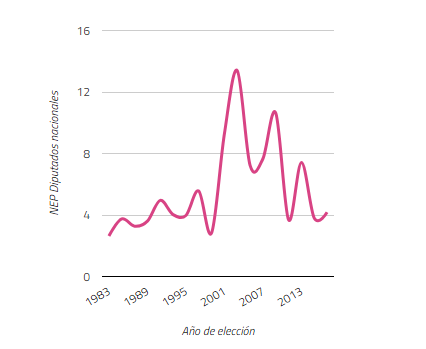
\includegraphics[scale=0.675]{grafico2}
    \caption{Número efectivo de partidos, Diputados (Fuente: CIPPEC)}
    \label{fig:1}
  \end{figure}
    \end{frame}


    
 \begin{frame}\frametitle{Poder legislativo: Fragmentación (cont.)}
 \begin{figure}[htbp]
    \centering
    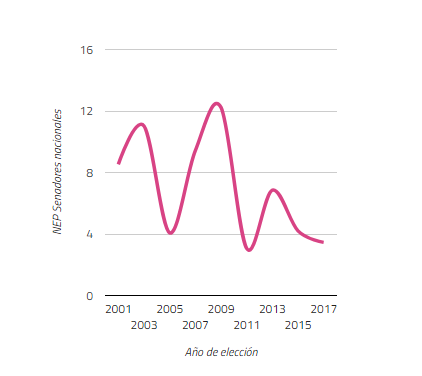
\includegraphics[scale=0.625]{grafico3}
    \caption{Número efectivo de partidos, Senadores (Fuente: CIPPEC)}
    \label{fig:1}
  \end{figure}
    \end{frame}




    
    

  \begin{frame}\frametitle{Poder legislativo: Reglas electorales (cont.)}
    \begin{itemize}
    \item Otra característica importante es si la elección de
      representantes se hace a través de \textbf{listas cerradas} o
      \textbf{listas abiertas}.
      \item En el primero, los líderes partidarios
      controlan los componentes y el orden en la lista. En el segundo,
      los lideres partidarios tienen poco control sobre quíen y en qué
      orden termina en la lista.
      \item En el primer caso, se fortalece la disciplina partidaria
        pero a costa de lesionar el accountability vertical; en el
        segundo caso pasa lo contrario. 
    \end{itemize}
    \end{frame}
    



  \begin{frame}\frametitle{Poder legislativo: Reglas electorales (cont.)}
    \begin{itemize}
    \item Los sistemas uninominales privilegian las coaliciones
      pre-electorales, mientras que los plurinominales favorecen las
      coaliciones post-electorales.
      \item Un sistema intermedio es aquel con distritos binominales
        (Chile) en el que se favorecen las coaliciones pre-electorales
        (no de gobierno sino coaliciones electorales); el sistema
        binomial favorece la estabilidad de las coaliciones
        \item Si además, los costos de entrada son bajos (Argentina),
          resulta dificil articular coaliciones duraderas y estables
          lo cual promueve en general politicas más estables
    \end{itemize}
    \end{frame}


  \subsection{Gobierno: Poder judicial}

   \begin{frame}\frametitle{Poder judicial}
    \begin{itemize}
    \item Sistema judicial definido por
      adopción del sistema de derecho romano (civil law) o anglosajón
      (common law)
      \item El poder judicial puede jugar diferentes roles en el
        contexto de las políticas públicas de un país:
        \begin{itemize}
        \item Puede ser un \textit{arbitro imparcial}
          $\longrightarrow$ preserva la durabilidad y estabilidad de
          las políticas
          \item Puede ser un \textit{jugador} $\longrightarrow$ que
            moldea las políticas de acuerdo a sus preferencias y las
            de la sociedad
          \end{itemize}
          \item Relevancia del poder judicial como un actor más del
            juego político depende del grado de independencia judicial
            $\longrightarrow$ podrá desempeñar su rol reactivo y
            proactivo de mejor manera mientras más independiente.  
      \end{itemize}
    \end{frame}
    



    
  \section{Burocracia}

  \begin{frame}\frametitle{Burocracia}
    \begin{itemize}
    \item Tipos y características de las burocracias afectan la
      calidad de las políticas públicas no sólo el diseño sino su implementación
      \item Dos factores relevantes son: el \textbf{grado de
          autonomía} --independencia del gobierno- y las
        \textbf{capacidades técnicas} --compensación y evaluación
      \item Se pueden pensar cuatro tipos de burocracias:
        \begin{itemize}\itemsep 5pt
        \item Meritocráticas $\longrightarrow$ altos
          niveles de autonomía y capacidad
          \item Clientelares $\longrightarrow$ bajos
            niveles de autonomía y capacidad
            \item Administrativas $\longrightarrow$ alta
              autonomía pero baja capacidad
              \item Paralelas $\longrightarrow$ baja
                autonomía y alta capacidad
          \end{itemize}
      \end{itemize}
    \end{frame}


 \begin{frame}\frametitle{Burocracia (cont.)}
    \begin{itemize}
    \item Evidencia de que es dificil realizar reformas sostenidas del
      servicio civil en muchos países $\longrightarrow$ caso de países
      latinoamericanos estudiado por Geddes.
      \item Cuando los países dependen mucho de ``votos clientelares''
        y la sociedad no asigna un gran valor a los políticos
        reformistas, entonces existe una gran dificultad para
        sancionar reformas que avancen en ese sentido
        \item Finalmente, una burocracia meritocrática en general
          tiene varias ventajas una de las cuales es dar mayor
          previsibilidad y continuidad a las políticas. 
      \end{itemize}
    \end{frame}


\begin{frame}\frametitle{Burocracia (cont.)}
 \begin{figure}[htbp]\vspace{0cm}
    \centering
    \includegraphics[scale=0.25]{burocracia1}
    \caption{Mérito de la burocracia. Fuente: BID en base a 18 países
      de Latam}
    \label{fig:1}
  \end{figure}
        \end{frame}
    


\begin{frame}\frametitle{Burocracia (cont.)}
 \begin{figure}[htbp]\vspace{0cm}
    \centering
    \includegraphics[scale=0.25]{burocracia2}
    \caption{Capacidad funcional burocrática. Fuente: BID en base a 18
    países de Latam}
    \label{fig:1}
  \end{figure}
        \end{frame}




\begin{frame}\frametitle{Burocracia (cont.)}
 \begin{figure}[htbp]\vspace{0cm}
    \centering
    \includegraphics[scale=0.25]{burocracia3}
    \caption{Tamaño y calidad de la burocracia. Fuente: BID en base a 18
    países de Latam}
    \label{fig:1}
  \end{figure}
        \end{frame}



        
\begin{frame}\frametitle{Burocracia (cont.)}
 \begin{figure}[htbp]\vspace{-0.5cm}
    \centering
    \includegraphics[scale=0.4]{burocracia4}
    \caption{Tipos de burocracia. Fuente: BID en base a 18
    países de Latam}
    \label{fig:1}
  \end{figure}
        \end{frame}

        

        

  \section{Grupos de interés}
   
\begin{frame}\frametitle{Grupos de interés}
\begin{itemize}\itemsep 15pt
\item  Los grupos de interés son agrupaciones de personas y/o empresas
  que se organizan al margen del proceso electoral para tratar de
  influir a favor de sus intereses en las decisiones de política
\item Se diferencian de los votantes en que tienen un alto grado de
  organización y coordinación; detectan polizones (free-riders)
  facilmente. Los intereses son homogéneos, suelen tener pocos
  miembros. 
\end{itemize}
\end{frame}



\begin{frame}\frametitle{Grupos de interés: Acciones}
\begin{itemize}\itemsep 5pt
\item Contribuciones y fondos de campaña a partidos/candidatos (epoca
  de campaña) $\longrightarrow$ obviamente esto introduce una
  asimetría de poder entre votantes y grupos de interés
\item Suministran información a los votantes a través de medios y
  actos $\longrightarrow$ esto supone que existe una asimetría de
  información entre el gobierno y los votantes
\item Audiencias de intereses $\longrightarrow$ los intereses
  organizados frecuentemente se reunen con representantes del
  ejecutivo y legislativo $\longrightarrow$ ``comprar acceso''.
  \item Conexiones y vínculos preexistentes --ie. empresas, colegios,
    etc. 
\end{itemize}
\end{frame}


\begin{frame}\frametitle{Grupos de interés: Acciones (cont.)}
 \begin{figure}[htbp]\vspace{-1cm}
    \centering
    \includegraphics[scale=0.35]{grupos1}\vspace{-0.75cm}
    \caption{Tipos de acciones realizadas por grupos de interés}
    \label{fig:1}
  \end{figure}
        \end{frame}


\section{Votantes}

\begin{frame}\frametitle{Votantes}
\begin{itemize}\itemsep 15pt
\item Los votantes deciden a quien votar en función de qué
  partido se acerca más a sus intereses y --a priori- votan
  al partido que propone una política más cercana a sus
  intereses
\item Para decidir si emite el sufragio, el votante considera los
  beneficios y costos de ir a votar
\begin{equation}
u_i=f(ben;dd;c)
\end{equation}
\item donde $ben$ es el beneficio asociado a que gane el
  partido preferido; $dd$ es el beneficio asociado al voto
  como deber democrático; y $c$ es el costo asociado de ir a votar. 
\end{itemize}
\end{frame}



    

\section{Competencia electoral: Grupos de interés}


\begin{frame}\frametitle{Aproximaciones teóricas}
\begin{itemize}\itemsep 15pt
\item Existen dos modelos teóricos fundacionales del análisis de
  competencia electoral con grupos de interés: el modelo de Baron y el
  modelo de Grossman \& Helpman. 
\begin{itemize} \itemsep 15pt \medskip 
\item Modelo de Baron $\longrightarrow$ 
\item Modelo de Grossman \& Helpman $\longrightarrow$
\end{itemize}
\item A diferencia de Downs-Black, ambos modelos suponen que
  \underline{no todos} los votantes conocen las posiciones de política
  de los candidatos (que pasa si todos estan informados?)
\end{itemize}
\end{frame}


\begin{frame}\frametitle{Modelo de competencia electoral de Baron}
\begin{itemize}\itemsep 15pt
\item Se suponen dos tipos de votantes: \textit{informados} y
  \textit{no informados}. Los gastos de campaña influencian el voto de
  los votantes no informados.
\item Al haber candidatos no informados, los partidos pueden tener
  incentivos para separar sus posiciones de política y atraer grupos
  de interes $\longrightarrow$ polarización de políticas
\item De alguna manera, esto equivale a proponer que los partidos
  compiten en un juego de suma cero por los votantes no informados. 
\item El modelo propone dos casos: 1) Política particularista
  $\longrightarrow$ beneficios a GIS y se niega a no contribuyentes;
  2) Política colectiva $\longrightarrow$ afecta a todos los GIS
  independientemente de si contribuyen. 
\end{itemize}
\end{frame}


\begin{frame}\frametitle{Modelo de competencia electoral de Baron}
\begin{itemize}\itemsep 15pt
\item Los partidos/candidatos compiten por votos y contribuciones de
  campaña a lo largo de varias dimensiones:
\begin{itemize}\itemsep 15pt \medskip 
\item Servicios de \textit{constituency}
\item Políticas mayoritarias
\item Políticas particularistas
\item Políticas colectivas
\end{itemize}
\item Las dos primeras no tienen un vínculo directo con grupos de
  interes especial. Las dos ultimas, si. 
\end{itemize}
\end{frame}


\begin{frame}\frametitle{Modelo de competencia electoral de Baron
    (cont.)}
\begin{itemize}\itemsep 15pt 
\item ¿Qué son políticas particularistas y políticas colectivas?
\begin{itemize}\itemsep 15pt \medskip
\item Políticas particularistas $\longrightarrow$ dan beneficios a
  \textit{algunos} GIS e imponen costos no significativos sobre otros
  GIS --no induce a hacer contribuciones. Ejemplos: excepciones
  regulatorias; provisiones especiales; recorte impositivo; acceso al candidato. 
\item Políticas colectivas $\longrightarrow$ dan beneficios
   significativos a \textit{algunos} GIS e imponen costos
   significativos a \textit{otros} GIS --si induce a hacer
   contribuciones. Ejemplos: legislación laboral; política comercial
   que afecta a importaciones y exportaciones; política tributaria
   amplia. 
\end{itemize}
\item Resumiendo $\longrightarrow$ políticas colectivas activan
  contribuciones de \textit{todos} los GIS. Las políticas
  particularistas no y adicionalmente generan un trade-off entre
ir al centro/los extremos. 
\end{itemize}
\end{frame}



\begin{frame}\frametitle{Modelo de competencia electoral de Baron (cont.)}
\begin{figure}[htbp]
    \centering \vspace{-3.5cm}
    \includegraphics[scale=0.52]{baron2}
    \caption{Políticas, beneficios y costos}
    \label{fig:baron1}
  \end{figure}
\end{frame}


\begin{frame}\frametitle{Modelo de competencia electoral de Baron
    (cont.)}
\begin{itemize}\itemsep 15pt 
\item ¿Cuáles son las implicancias para las contribuciones de campaña? 
\begin{itemize}\itemsep 15pt \medskip
\item Políticas particularistas $\longrightarrow$ contribuciones son
  sólo función de la política del candidato que favorece a ese GIS
  --$C_{i}=f(p^{A})$. Estas políticas pueden ser negadas a los GIS
\item Políticas colectivas $\longrightarrow$ contribuciones son
  función de las políticas de ambos candidatos
  --$C_{i}=f(p^{A};p^{B})$. No pueden ser negadas a los GIS
\item Las contribuciones pueden ser negadas en dos casos: 1) no hay
  ninguna contribución; 2) si un GIS dona a ambos candidatos. 
\end{itemize}
\end{itemize}
\end{frame}




\begin{frame}\frametitle{Modelo de competencia electoral de Baron (cont.)}
\begin{itemize}\itemsep 15pt
\item 1 dimensión, 2 partidos (candidatos). Cada partido asume una
  posición en una escala espacial --partido A entre 0 y 0.5 y partido
  B entre 0.5 y 1. Votantes de dos tipos: no informados (fraccion
  \textit{k})e informados (fracción \textit{1-k}). 
\item El mediano de los votantes informados prefiere posiciones de
  candidatos ubicadas al centro de la dimensión política. La presencia de
  votantes informados crea \textit{incentivos centripetos}
\item Votantes no informados desconocen posiciones de políticas
  $\longrightarrow$ persuadidos por campaña. Los candidatos gastan
  $C1,C2$ para atraer votantes no informados. Las contribuciones crean
  \textit{incentivos centrífugos} 
\item La probabilidad de ganar $W1$ es funcion directa de $C1$ e
  indirecta de $C2$ --$W_{1}=f(C_{1};C_{2})$. 
\end{itemize}
\end{frame}


\begin{frame}\frametitle{Modelo de competencia electoral de Baron
    (cont.)}
\begin{itemize}\itemsep 15pt
\item La probabilidad de ganar es mayor para el partido alineado con
  el GIS que mas valua las políticas particularistas.
\item Si la proporcion de votantes no informados aumenta, las
  políticas de equilibrio divergen y se mueven fuera del centro
\item Si existe también financiamiento público, resultara en políticas
  particularistas mas cercanas al mediano --financiamiento público
  realza los incentivos centripetos.
\item Adicionalmaente, financiamiento público tiene una caracteristica
  de tipo ``underdog'' $\longrightarrow$ aumentos en financiamiento
  público aumentan la probabilidad de ganar del candidato con menor
  chances. 
\end{itemize}
\end{frame}



\begin{frame}\frametitle{Modelo de competencia electoral de Baron (cont.)}
\begin{figure}[htbp]
    \centering \vspace{-3.5cm}
    \includegraphics[scale=0.44]{baron1}
    \caption{La secuencia del juego de la competencia electoral}
    \label{fig:baron1}
  \end{figure}
\end{frame}



\begin{frame}
\frametitle{Modelos de lobbies}
\begin{itemize} \itemsep 10pt
\item Modelo estándar de lobies de grupos de interés
  especial (SIG) es de Grossman \& Helpman. Gobiernos de
  tipo oportunista, votantes con interés medio $v$ y grupos de interés
  con interés medio $c$. 
\item Sin SIG's el gobierno implementaría una
  política acorde al interés del votante mediano; con la presencia de
  SIG's el gobierno tiene un incentivo a apartarse de esa política. 
\item Resultados electorales son influidos (al menos en parte) por
  el dinero gastado por los candidatos en las campañas --atraen a
\textit{swing voters} a la Baron (1994) y Grossman \& Helpman (1996).
\end{itemize}
\end{frame}


\begin{frame}
\frametitle{Modelos de lobbies (cont.)}
\begin{itemize}
\itemsep 10pt
\item Supuesto principal $\longrightarrow$ individuos pueden organizarse e ``influenciar'' sobre políticos y/o partidos para obtener políticas deseadas --i.e. lobbies del azúcar en EEUU, grupos de interés sectoriales, lobbies de grupos financieros, etc.
\item Supuestos operativos (artículo Grosman \& Helpman (1992):
\begin{enumerate}
\item $n$ grupos de agentes --tamaño de cada grupo igual a 1
\item Preferencias idénticas hacia adentro del grupo
\item Vector de políticas $\longrightarrow$ $q$. La política es elegida por el político.
\item Los lobbies realizan transferencias (aportes, coimas, etc) para influir sobre la política
\item Utilidad de los agentes lineal en el consumo
\end{enumerate}
\end{itemize}
\end{frame}


\begin{frame}
\frametitle{Modelos de lobbies (cont.)}
\begin{equation}
W_j(q)-C_j(q)
\end{equation}
\begin{itemize}
\item $W_j(q)$ es el ingreso del grupo lobby y $C_j(q)$ es el consumo (transferencias) realizado. Note como tanto el ingreso como las transferencias del lobby son funciones de las políticas adoptadas.
\end{itemize}
\begin{equation}
G(q)=\sum_{i=1}^n C_j(q)+\alpha \sum_{i=1}^n W_j(q)
\end{equation}
\begin{itemize}
\item es la función de utilidad del político; depende en forma lineal de las transferencias recibidas y del bienestar agregado (suma de ingresos). Note la importancia del parámetro $\alpha$: denota lo mucho o lo poco que le importa el bienestar general al político
\end{itemize}
\end{frame}


\begin{frame}
\frametitle{Modelos de lobbies (cont.)}
\begin{itemize}
\item $m$ grupos ($m < n$) están organizados como lobbies; el remanente $n-m$ no están organizados y no hacen ningún tipo de contribución
\item Forma del juego:
\begin{enumerate}
\item Todos los lobbies organizados ofrecen \textit{simultáneamente} una propuesta $C_j(q)>0$ que representan los pagos que harían a los políticos cuando la política $q$ es implementada. 
\item Los políticos observan las propuestas y luego deciden (implementan) la política $q$. 
\end{enumerate}
\item El juego tiene la misma forma que un juego de subastas (de ahí en parte el nombre del artículo ``Protection for sale'')
\end{itemize}
\end{frame}


\begin{frame}
\frametitle{Modelos de lobbies (cont.)}
\begin{proposition}
La función de contribuciones $\{C_j^*(.)\}_{j=1,..m}$ y la política $q^*$ constituyen un equilibrio de subjuego de Nash si y sólo si:
\begin{enumerate}
\item $C^*_j(.)$ es viable $\longrightarrow$ $0 \leq C^*_j(q) \geq W_j(q)$
\item El político elige la política que maximiza su bienestar:
\begin{equation}
q^* \in \arg\max_q \sum_{j=1}^m C_j^*(q)+\alpha \sum_{j=1}^n W_j(q)
\end{equation}
\item Ningún lobby puede beneficiarse de desviaciones alternativas
\begin{equation}
q^* \in \arg\max_q (W_i(q)-C^*_i(q)+ \sum_{j=1}^m C_j^*(q)+\alpha \sum_{j=1}^n W_j(q))
\end{equation}
\end{enumerate}
\end{proposition}
\end{frame}


\begin{frame}
\frametitle{Modelos de lobbies (cont.)}
Además, debe verificarse que:
\begin{equation}
q^j \in \arg\max_q (\sum_{j=1}^m C_j^*(q)+\alpha \sum_{j=1}^n W_j(q))
\end{equation}
\begin{itemize}
\item es decir, que existe una política $q^j$ para cada lobby y que además satisfaga $C^*_j(q^j)=0$. Esto implica que la función de contribuciones de cada lobby es tal que existe una política asociada a contribuciones cero y sin embargo le brinda la misma utilidad
\item Si la condición 3 no se da, quiere decir que existe un $\hat{q} \neq q^*$ que le brindará una mayor utilidad al político y $q^*$ no sería un equilibrio en ese caso.
\end{itemize}
\end{frame}


\begin{frame}
\frametitle{Modelos de lobbies (cont.)}
\begin{itemize}
\item Pero poco sabemos acerca de la(s) propuesta(s) de contribucion(es). Tomando la derivada de las ecuaciones (9) y (10), tendremos que:
\begin{align}
\sum_{j=1}^m \frac{\partial C_j^*(q)}{\partial q_K} + \alpha \sum_{j=1}^n \frac{\partial W_j(q)}{\partial q_K} \\
\frac{\partial W_i(q)}{\partial q_K}- \frac{\partial C_i^*(q)}{\partial q_K}+\sum_{j=1}^m \frac{\partial C_j^*(q)}{\partial q_K} + \alpha \sum_{j=1}^n \frac{\partial W_j(q)}{\partial q_K}
\end{align}
\item lo cual nos queda:
\begin{equation}
\frac{\partial W_i(q)}{\partial q_K} = \frac{\partial C_i^*(q)}{\partial q_K}
\end{equation}
\end{itemize}
\end{frame}


\begin{frame}
\frametitle{Lobbies: ejemplo de aplicación}
\begin{itemize}
\item Dos grupos: ricos y pobres. Una fracción $\lambda$ de los agentes son ricos con ingreso $h^r$ y los restantes $1-\lambda$ son pobres, $h^p (<h^r)$. El ingreso promedio en la economía es:
\begin{equation}
h=\lambda h^r + (1-\lambda)h^p 
\end{equation}
\item Se impone un impuesto $\tau$ a todos los agentes y se redistribuye el producido con subsidios de suma fija. La existencia de impuestos ocasiona una pérdida, $c(\tau)h$, y $c(\tau)$ es creciente y convexa. El monto total del subsidio es:
\begin{equation}
\Gamma=(\tau-c(\tau))h
\end{equation} 
\end{itemize}
\end{frame}


\begin{frame}
\frametitle{Lobbies: ejemplo de aplicación (cont.)}
\begin{itemize}
\item Con votación por mayoría, tendremos la tasa impositiva preferida por los pobres (son más numerosos):
\begin{equation}
\tau^m= \arg\max_{\tau} (1-\tau)h^p+[\tau-c(\tau)]h
\end{equation}
\item Maximizando, queda:
\begin{equation}
h-h^p=c'(\tau^m)h
\end{equation}
\item mientras $h-h^p$ sea mayor que $\epsilon$ tendremos que $\tau^m>0$ y habrá redistribucion
\end{itemize}
\end{frame}


\begin{frame}
\frametitle{Lobbies: ejemplo de aplicación (cont.)}
\begin{itemize}
\item Supongamos ahora que los ricos se organizan en un lobby. La tasa impositiva de equilibrio será:
\begin{align}
\tau^l= \arg\max_{\tau}  (1+\alpha)\lambda[(1-\tau)h^r+[\tau-c(\tau)h]+ \\ 
\alpha(1-\lambda)[(1-\tau)h^p+[\tau-c(\tau)h]  
\end{align}
\item La CPO queda igual a:
\begin{equation}
\lambda[h-h^r-c'(\tau^l)h]-\alpha c'(\tau^l)h \leq 0
\end{equation}
\item y como $h-h^r<0$, tendremos que $\tau^l=0$. Con lobby, no hay lugar para imposición redistributiva. Este mismo resultado se para cuando los pobres también están organizados. Implicancia $\longrightarrow$ si la imposición es costosa, la política maximizadora de utilidad es una política de cero impuestos
\end{itemize}
\end{frame}


\begin{frame}
\frametitle{Lobbies: ejemplo de aplicación (cont.)}
\begin{itemize}
\itemsep 15pt
\item Ahora supongamos que la redistribución es socialmente deseada (i.e. contribuye a la formación humana via transferencias a los más pobres). Esto sugiere que $c'(\tau)<0$ para $\tau \leq \hat{\tau}$ y que $c'(\hat{\tau})=0$. En este caso, la política maximizadora  de utilidad será $\tau=\hat{\tau}$
\item Con los ricos organizados, igualmente tendremos que no habrá redistribución. Esto sugiere que con el sector rico organizado, el resultado encajará mejor con sus preferencias; entonces, políticas que redistribuyen desde ricos a pobres no serán adoptadas aún cuando sean socialmente benéficas. 
\end{itemize}
\end{frame}


  \begin{frame}\frametitle{Evidencia: votante swing, tecnología y política}
          \begin{itemize}\itemsep 15pt
          \item Tradicionalmente, idea teórica es que las elecciones
            se definen por los indecisos $\longrightarrow$ ``swing
            voters''
            \item En EEUU, este porcentaje era de 20\% en 1990, de
              10\% en 2000 y de 5\% en 2016.
              \item Big data y tecnología facilita y abarata el
                ``micro-targeting''.
                \item El foco pasa a ser el votante core y no el
                  votante swing. 
            \end{itemize}
\end{frame}


  \begin{frame}\frametitle{Evidencia: votante swing, tecnología y
      política (cont.)}
   \begin{figure}[htbp]
    \centering
    \includegraphics[scale=0.5]{figura3}
\caption{Los ``medianos'' de cada partido. Fuente: Pew Research Center}
  \end{figure}
          \end{frame}



              \begin{frame}\frametitle{Evidencia: votante swing en Argentina}
 \begin{itemize}\itemsep 15pt
          \item La tendencia parece ser al revés! $\longrightarrow$
            según diferentes encuestas, a una semana de la elección
            presidencial de 2015, entre un 15\% y 20\% aún no habían decidido su
            voto
            \item Está pasando en otras democracias multi-partidistas
              $\longrightarrow$ mas de dos opciones electorales
              \item El foco es el votante swing? No está claro, pero
                la tendencia indica que puede ser decisivo.
            \end{itemize}
            \end{frame}



  
\end{document}
  